\documentclass[11pt]{article}
\usepackage{icmlko}
\begin{document}

\title{일곱 자리 중 둘 --- 전이의 0.39 가 어디 앉아 있나}
\author{월드모델 실험실}
\date{노트 424 · 2026년 8월 3일}
\maketitle

\begin{abstract}
노트 423이 도메인 표지의 \textbf{재료}가 전이의 전부임을 보였다 ---
같은 구조에 field 만 바꾼 \texttt{grp2} 가 KR 만화 전이를
$+0.1970 \to -0.1918$ 로 뒤집는데 판은 $0.0005$ 밖에 안 다르다.
그러면 물어야 할 것은 \textbf{어느 자리인가}다.

일곱 자리를 하나씩만 바꿔 쟀다(나머지는 \texttt{grp} 그대로).

\begin{center}
\begin{tabular}{llr}
\hline
바꾼 자리 & 새 field & 기준 대비 \\
\hline
\textbf{모바일} & \texttt{advisory} & $\mathbf{-0.1182}$ \\
\textbf{펀딩} & \texttt{adult\_only} & $\mathbf{-0.1128}$ \\
애니 & \texttt{is\_original} & $-0.0262$ \\
세계애니 & \texttt{source} & $-0.0231$ \\
웹툰 & \texttt{daily\_pass} & $-0.0021$ \\
게임 & \texttt{n\_platform} & $+0.0000$ \\
도서 & \texttt{book\_format} & $+0.0055$ \\
\hline
\end{tabular}
\end{center}

\textbf{두 자리가 합의 83\% 를 낸다.} 나머지 다섯은 다 합쳐도 $-0.046$ 이다.
하나씩의 합은 $-0.277$ 이고 전부 바꿨을 때는 $-0.386$ --- \textbf{어울림이
조금 있지만 자리별 몫이 대부분}이다.

\textbf{전이를 사고파는 자리는 일곱이 아니라 둘이다.}
\end{abstract}

\section{균형은 아니다}

제일 그럴듯한 설명부터 쟀다 --- \emph{표지가 한 무리로 쏠리면 사실상 표지가
없어진다.} 무리 수 · 최대 몫 · 엔트로피를 다 재고 손해와 견줬다.

\begin{center}
\begin{tabular}{lrr}
\hline
 & $\rho$ (손해와) \\
\hline
최대 몫 변화 & $-0.143$ \\
엔트로피 변화 & $+0.000$ \\
\texttt{grp2} 쪽 최대 몫 & $+0.143$ \\
\hline
\end{tabular}
\end{center}

\textbf{전부 0 근처다.} 자료를 보면 왜 안 되는지 바로 보인다 --- 두 큰
손해가 \textbf{반대 방향}으로 움직인다.

\begin{itemize}
\item 펀딩: \texttt{category}(21무리 · 엔트로피 $2.765$) $\to$
\texttt{adult\_only}(한 무리가 $99.2\%$ · 엔트로피 $0.048$). 표지가
\textbf{사실상 없어진다} --- 읽힌다.
\item 모바일: 무료 여부(2무리 · 최대몫 $0.645$) $\to$
\texttt{advisory}(4무리 · 최대몫 $0.476$). \textbf{더 고르게 갈리는데}
제일 크게 잃는다 --- 안 읽힌다.
\end{itemize}

그리고 ``표지를 잃어서''로도 다 안 된다: 애니의 \texttt{is\_original} 은
한 무리가 $99.5\%$ 인데 $-0.026$ 밖에 안 잃는다. \textbf{펀딩과 애니가
같은 모양인데 손해가 네 배 다르다.}

\section{그래서 지금 말할 수 있는 것}

\textbf{말할 수 있는 것}: 전이의 $0.39$ 는 일곱 자리에 고르게 퍼져 있지
않고 \textbf{두 자리에 앉아 있다}. 모바일과 펀딩의 표지를 무엇으로 하느냐가
안 본 도메인의 성적을 정한다. 나머지 다섯은 바꾸든 말든 거의 같다.

\textbf{말할 수 없는 것}: 왜 그 둘인지. 균형은 아니고, 표지 상실만으로도
아니다. 노트 401 이후로 이 실험실은 $n{=}7$ 짜리 눈짐작을 안 짓는다.

\section{남은 것}

\begin{tabular}{lp{7.0cm}}
\hline
위쪽을 재 본다 & 지금까지는 \textbf{나쁘게 바꾸는} 것만 쟀다. 모바일·펀딩
자리에 \emph{다른} field 를 넣어 $+0.1946$ 을 \textbf{넘는지} 보는 것이
값이 있는 쪽이다 \\
펀딩 \texttt{category} 가 제일 센 표지 & 21무리 · 엔트로피 $2.765$ 로
일곱 중 제일 풍부하다. 다른 도메인에도 그만큼 풍부한 자리가 있나 \\
모바일 & 두 설명이 다 안 듣는 자리. 웹툰(노트 414)과 같은 종류의 숙제 \\
\hline
\end{tabular}

\begin{figure}[h]
\centering
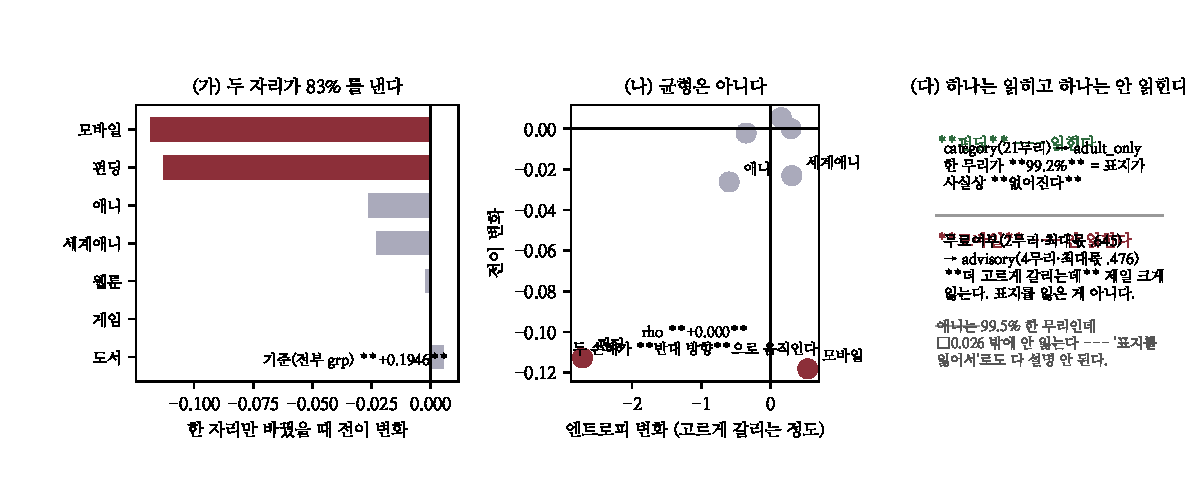
\includegraphics[width=\textwidth]{figs/fig424.pdf}
\caption{(가) 두 자리가 대부분을 낸다. (나) 균형 변화와 손해는 무관하다
($\rho = +0.000$). (다) 펀딩은 읽히고 모바일은 안 읽힌다.}
\end{figure}

\end{document}
